\documentclass[conference]{IEEEtran}
\usepackage{graphicx}
\usepackage{amsmath}
\usepackage{cite}
\usepackage{float}  

\title{A Technical Report on Wireless Site Survey and Architecture of Roaming for Wireless Access Networks in Commercial Areas.}

\author{
    \IEEEauthorblockN{Nguyen Duc Chi Dat}
    \IEEEauthorblockA{
        \textit{Faculty of Information Security,} \\
        \textit{University of Information Technology}\\ 
        Ho Chi Minh City, Viet Nam \\
        datndc.19@grad.uit.edu.vn
    }
}

\begin{document}

\maketitle

\begin{abstract}
This report investigates Wi-Fi coverage and signal strength at a specific area in Gigamall Shopping Center, Thu Duc, and explains the basic architecture of the network's roaming currently in use.
\end{abstract}

\begin{IEEEkeywords}
wireless site survey, roaming architecture, coverage analysis
\end{IEEEkeywords}

\section{Introduction}
Wireless site surveys are useful for ensuring good performance and coverage of Wi-Fi networks in equipped environments, especially in locations like shopping centers, as they require a stable Wi-Fi connection for a large number of users. Surveys should be conducted in small areas for more accuracy. This report aims to present findings and assess Wi-Fi signal strength, and coverage areas on the first floor of Gigamall Shopping Center, Thu Duc. These findings and assessments will serve as a basis for recommendations to enhance the network. Additionally, the report will explain the roaming architecture implemented to optimise connectivity across different areas within the network and improve overall user experience.
\section{Wireless Site Surveys}

\subsection{Site Description}
This area is the Gigamall Shopping Center in Thu Duc, frequently visited by local residents due to its many shopping and entertainment zones, as well as large supermarket systems. The surveyed floor is the first floor, covering an area of approximately 12,000 square meters. The layout consists of shops, stairs, and corridors. The walls are made of plastic partitions with a steel frame, and the doors are made of glass.

The survey was conducted on the weekend during peak hours. The highest density was recorded at Highland Coffee, where a large number of people gathered to relax.

\subsection{Methodology}
To ensure a thorough assessment of network conditions, a strategic selection of survey points was made. These points were carefully chosen to provide representative coverage across the entire mall, encompassing various areas such as common spaces, retail outlets, and food courts. A floor map was generated using data from the official Gigamall website. Network access points were identified and marked on the map. The next steps involved identifying the points to be surveyed; these selected points had to be specific locations to ensure that the survey covered nearly all aspects of the floor. To facilitate data collection, specialized network measurement tools were configured on mobile and laptop devices. 

Specifically, \textit{speedtest-cli} utility is used to quantify internet performance metrics, including upload and download speeds as well as network latency. Due to the large number of points to be surveyed, a Python script was utilized to automate the process and save the records into a text file whenever one of these points was reached. Moreover, \textit{lswifi} commandline tool was employed to list all the recognizable Wi-Fi networks within range, capturing essential details such as Service Set Identifiers (SSIDs), Received Signal Strength Indicators (RSSIs), channels, frequencies, security protocols, and 802.11 standards.

Given the substantial number of survey points, a Python script was developed to automate the data collection process. This script enabled the efficient recording of network measurements at each designated location, storing the results in a csv file for subsequent analysis.

Once preparations were complete, the next step was to walk through the marked locations and capture the necessary information. It was important to note the points where the device could switch from one access point to another. The collected data will be visualized using Microsoft Excel and Chart.js to generate graphical representations. The resulting visualizations will be presented in the subsequent section.

\subsection{Findings and Analysis}

Fig. 1 below is the heatmap illustrating the Wi-Fi signal strength received by the device across the floor, with four access points located at positions as shown on the map. Signal strength is visually represented by a color gradient, ranging from red (strongest signal) to orange, yellow, and blue (weakest signal).

\begin{figure}[htbp]
    \centering
    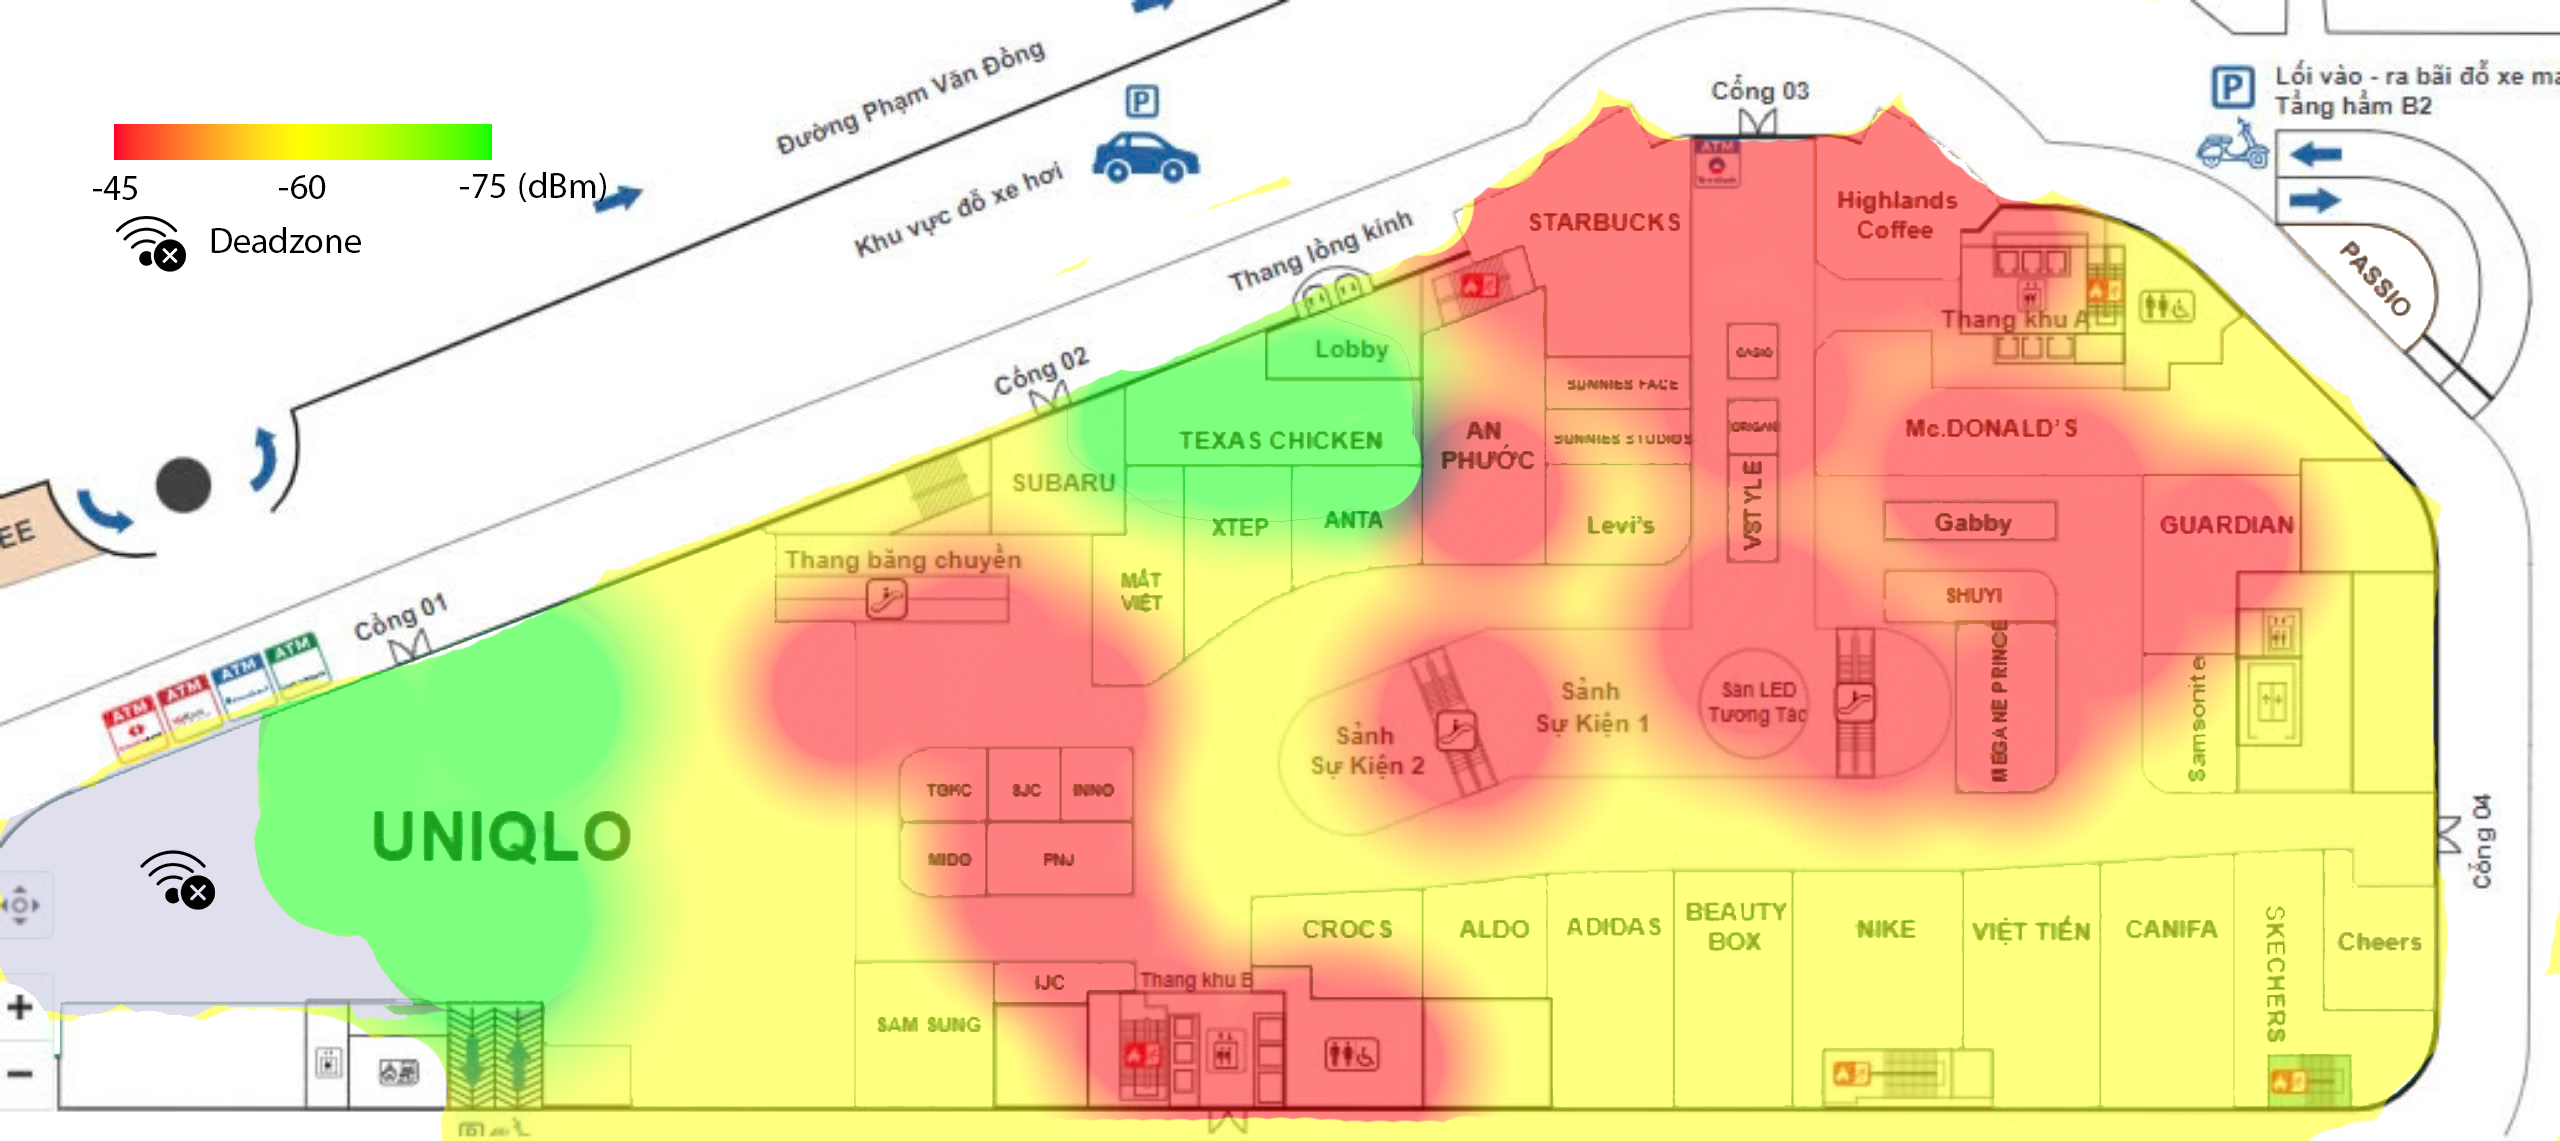
\includegraphics[width=0.48\textwidth]{fig1_heatmap.png}
    \caption{Heatmap of Wi-Fi signal coverage on the first floor of Gigamall Shopping Center.}
\end{figure}

The spacious central area on the map is a common space within the shopping mall, equipped with approximately 3 public Wi-Fi access points to meet the high demand of visitors for browsing, online shopping, and entertainment. As can be seen from the map, the signal in this area is always measured above -60 dBm, which was only sufficient at the time the survey was conducted. Within a 10-meter radius of each access point, a level below -60 dBm can be achieved. However, the stability is not high due to the large number of connections accessing simultaneously. Improving the signal strength would be beneficial to ensure more reliable and faster connections, especially during peak usage periods.

The surrounding areas are shop houses separated from the common space by walls, glass, and large plastic panels. Despite being within the shopping center, these shop houses suffer from poor Wi-Fi signal strength. Consequently, most shop houses have deployed their own Wi-Fi networks, leading to a dense Wi-Fi environment. This high density of Wi-Fi networks can result in interference, particularly when multiple networks operate on the same channel or frequency band (2.4GHz or 5GHz). As illustrated in Fig 2, signal strength typically decreases with distance from the access point, but factors such as physical obstructions, high density of Wi-Fi networks and a large number of concurrent connections can cause deviations from this general trend, resulting in non-monotonic chart values.

\begin{figure}[htbp]
    \centering
    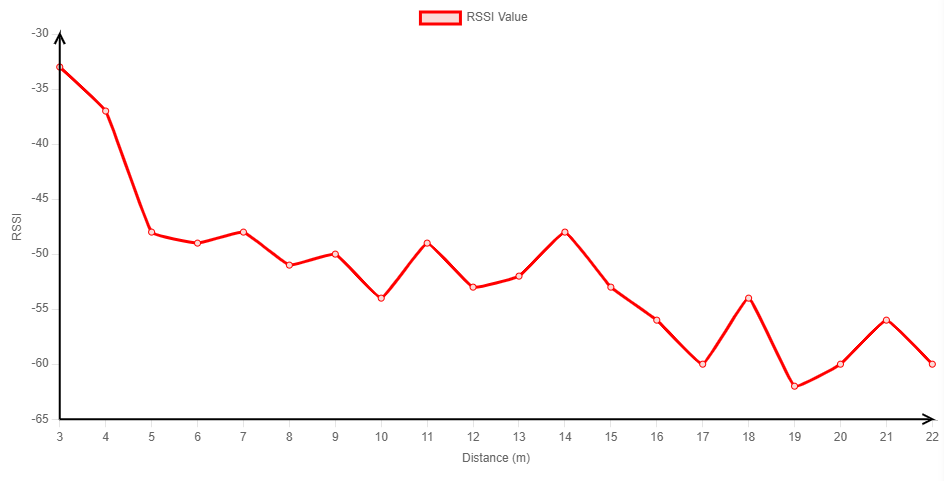
\includegraphics[width=0.48\textwidth]{fig2_rssi.png}
    \caption{A line chart shows the relationship between distance from access
point and RSSI.}
\end{figure}

Fig. 3 compares the signal strength under line-of-sight (LoS) and non-line of sight (Non-LoS) conditions. Signal strength measurements were collected over a 120-second interval while connected to the same access point at a fixed distance. As shown, the LoS condition consistently exhibits stronger signal strength and less attenuation compared to the Non-LoS condition.

\begin{figure}[htbp]
    \centering
    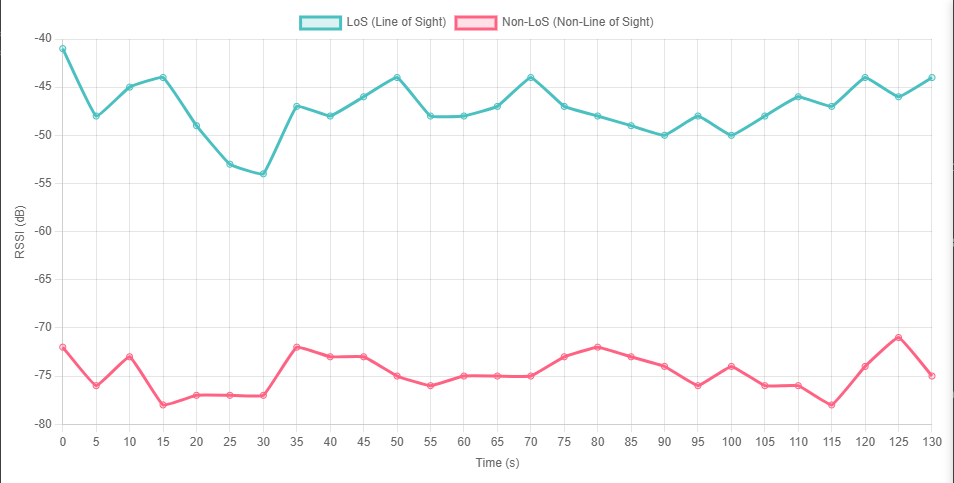
\includegraphics[width=0.48\textwidth]{fig3_los_nonlos.png}
    \caption{A graph illustrates signal strength in LoS and Non-LoS conditions.}
    \label{fig:los_nonlos}
\end{figure}

Additionally, data on upload and download speeds, as well as latency at each surveyed spot, are illustrated in Fig. 4. The green line represents latency in milliseconds (ms) on the right axis, while the red and blue bars represent upload and download speeds in Megabits per second (Mbps) respectively.

\begin{figure}[htbp]
    \centering
    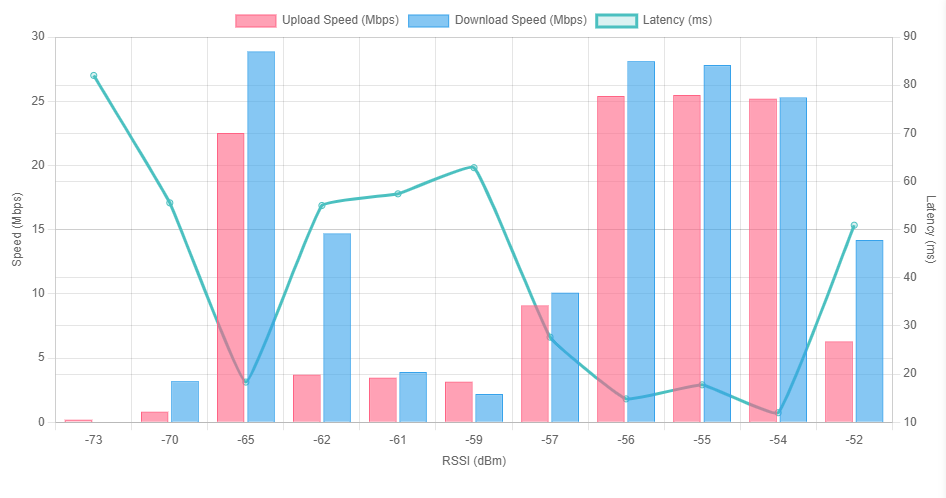
\includegraphics[width=0.5\textwidth]{fig4_speed_test.png}
    \caption{Relationship between distance from access point and RSSI.}
\end{figure}

The green line, representing latency, demonstrates an inverse correlation with RSSI. As signal strength (RSSI) diminishes, latency increases, and conversely. For instance, at low RSSI values (approximately -73 dBm), latency is elevated (above 70 ms), indicating a direct relationship between weak signal strength and increased data transmission delays. High latency potentially affects real-time applications like online gaming or video streaming.

As signal strength improves (higher RSSI values), both upload and download speeds increase. The peak upload and download speeds are achieved at RSSI values between -56 dBm and -54 dBm, with download speeds exceeding 25 Mbps and upload speeds reaching approximately 20 Mbps. Conversely, at weaker signal levels (e.g., -73 dBm), speeds are significantly reduced, approaching negligible levels. 

A clear correlation exists between stronger Wi-Fi signals (higher RSSI) and improved network performance, encompassing faster upload/download speeds and lower latency. The chart indicates that elevating signal strength, particularly above -60 dBm, can substantially enhance both speed and user experience by reducing latency. However, there are instances where the data deviates from the expected theoretical relationship due to the inherent instability of Wi-Fi signals as described in Fig. 2. A case in point is the anomalous spike in both download and upload speeds observed at an RSSI of -65 dBm.

The survey also identified two roaming areas where the access points overlapped and the device transitioned between access points without any signal interruption. Fig. 5 displays the changes in the access point BSSID, which is the MAC address of the access point, as the device moves into the roaming areas. Nonetheless, it discovered a dead zone where the Wi-Fi connection was disconnected before connecting to a new access point, indicating that the roaming transition in this area was not as smooth as expected. The reason for that situation is that the distance between the two access points is quite large, and signal strength is insufficient so the area cannot be fully covered. The roaming architecture will be discussed in more detail in section III.

\begin{figure}[htbp]
    \centering
    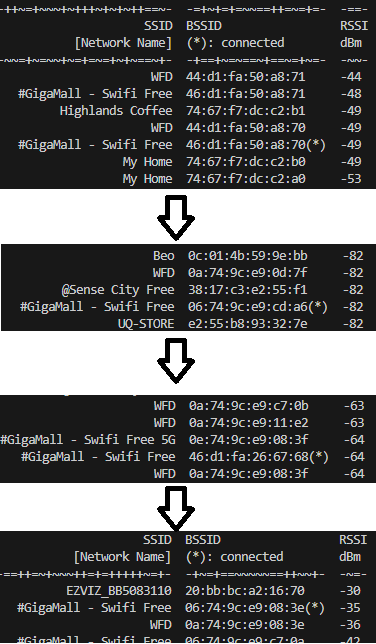
\includegraphics[width=0.44\textwidth]{fig5_rssid_change.png}
    \caption{An output demonstrates BSSID changes at each roaming spot.}
\end{figure}

\subsection{Recommendations for the network}

Based on the findings from the site survey, there are some suggestions to enhance the current network. First and foremost, placement of access points should be optimised and more access points should be installed in locations prone to interference. This study recommends installing four additional access points in the four rooms located at the centre of the floor to minimise dead zones in the rooms, assisting in increasing signal coverage to have a seamless roaming transition in these areas. These additional access points also help distribute the network load, reducing congestion on other access points. The proposed access point placement is shown in Fig. 6.

\begin{figure}[htbp]
    \centering
    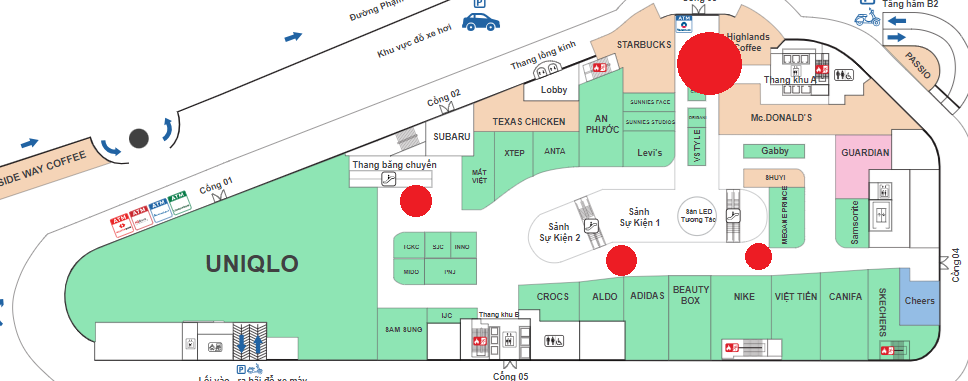
\includegraphics[width=0.4\textwidth]{acesspoint.png}
    \caption{A proposed access point placement.}
\end{figure}

Additionally, access points should be placed at higher elevations to improve signal distribution. When positioned higher, signals are less likely to be absorbed by people and objects, which can contribute to signal loss. Furthermore, a mesh Wi-Fi system that uses multiple nodes can be considered to be implemented to create a network with enhanced coverage, but its downside is that the speed is potentially reduced as the bandwidth is split. And importantly, more site surveys should be carried out regularly to evaluate progress as well as investigate if any spots require further improvements.

\section{Roaming Architecture}

This section will explain the meaning of roaming in wireless local area networks (WLANs), and introduce the basics of two types of roaming. It also describes the roaming model in the site survey.

\subsection{Definition of Roaming}
While joining a WLAN with multiple access points installed, the process by which a client device, also known as a wireless device, switches its connection from one access point to another access point as moving around the area is referred to as roaming \cite{article_example}.

Roaming in WLAN is categorised into two types: internal roaming and external roaming [2] [3]. The study only focuses on internal roaming since it is implemented in the area where the site survey was conducted.

\subsection{Internal Roaming}
Internal roaming or Layer 2 roaming refers to the process of connection is shifted between access points in the same network \cite{article_example}. Generally, the client device is not required to re-authenticate in internal roaming. The internal roaming process is shown in Fig. 7.

\begin{figure}[htbp]
    \centering
    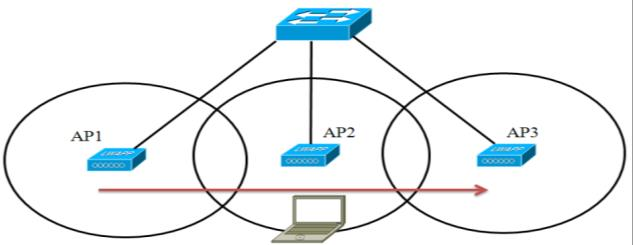
\includegraphics[width=0.4\textwidth]{internal_roaming.png}
    \caption{A picture displays the internal roaming (Layer 2 roaming) process
[4].}
\end{figure}

The client device, after participating in the network, will continuously listen for beacon frames or send probe requests to detect which access point has the strongest signal strength within its range and then decide to roam; the mechanism used to find access points is vendor-specific \cite{article_example}. Roaming can happen either when the signal strength of the current access point decreases or when detecting a higher signal strength level at another access point. The client device does not necessarily need to move into a designated or specific roaming spot; as long as it is within the overlapping range of access points, it can roam. In ideal cases, the roaming transition is seamless and no interruption of the data transmission between the client device and an application connected to the network occurs. However, there are also some situations where the client device disconnects from the current access point before re-associating with the new access point \cite{article_example} \cite{book_example}.

The process of internal roaming includes many steps other than just finding a new access point having a high RSSI to associate with. Roshan and Leary \cite{article_example} explain that there are some tasks for internal roaming as listed below and tasks with a mark (*) are not specified in the 802.11 standard so they are optional tasks.

\begin{itemize}
    \item The current access point must determine that the client has roamed away from it to the new access point.
    \item The current access point should temporarily store data any data meant for the roaming client. (*)
    \item The new access point must inform the current access point that the client has successfully roamed, typically through a unicast or multicast packet sent from the current access point to the new access point, using the client's MAC address as the source. (*)
    \item The current access point should forward the buffered data to the new access point. (*)
    \item The access points need to update the MAC address tables on the infrastructure switches to prevent data loss for the roaming client. (*)
\end{itemize}


To give an example of internal roaming, the UIT network in the site survey above uses internal roaming, as the SSIDs of the access points are similar—UIT Public, the IP address of the device was not changed when moving to another access point. As mentioned earlier, there are locations where the roaming process was seamless and others where connections were interrupted during roaming. Fig. 8 demonstrates how seamless roaming works in the site survey.

\begin{figure}[htbp]
    \centering
    \includegraphics[width=0.4\textwidth]{survey.png}
    \caption{An illustration of how seamless roaming works in the site survey.}
\end{figure}


\subsection{External Roaming}

External roaming, or Layer 3 roaming, in contrast to internal roaming, refers to the process of changing the connection between access points in different networks. It happens when the client device moves to another WLAN or even another internet service provider \cite{article_example}. This type of roaming is typically applied in large networks. During the external roaming process, the device involved must change its IP address \cite{article_example}. Fig. 9 below depicts the external roaming process.

\begin{figure}
    \centering
    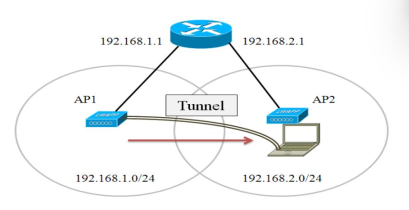
\includegraphics[width=0.5\textwidth]{fig9.png}
    \caption{An image represents the external roaming (Layer 3 roaming) process [4]}
    \label{fig:enter-label}
\end{figure}

\section{Conclusion}
This study has explored weak points of wireless network in the area through a site survey and the roaming architecture implemented. Besides, the importance of conducting a site survey is highlighted also. The data collected during the site survey supplies a basis for suggesting improvements to enhance signal coverage and reduce interference, helping design an effective wireless network that meets the needs of students, faculty, and staffs.

Additionally, the definition and classification of roaming introduced in the report provide insight into how to maintain seamless connectivity across different access points, improving overall network performance and user experience in the academic environment.

\bibliographystyle{IEEEtran}
\bibliography{references}

\end{document}
